\chapter{MATERIALS AND METHODS}
In this thesis, we predict the binding affinity score of drug-target pairs by using heterogeneous graphs generated with the existing and extracted information of chemicals and proteins. To do so, we divide the study in to 5 stages; in Stage 1, we compiled data from databases listed in Chapter \ref{chapter:dataset_preparation}, in Stage 2, we assembled these data as described in Section \ref{section:data_assembling} and extract useful information from them, in Stage 3, we created homogeneous and heterogeneous graphs using assembled data, in Stage 4, we learned the distributional vector representations of proteins and ligands using homogeneous and heterogeneous graphs with and without several language models, and finally in Stage 5, we predict the affinity scores of drug-target pairs, and  evaluate the performance of our model.

\section{Dataset Compilation}
% TO DO: Insert datasets chart here.
\begin{figure}
    \centering
        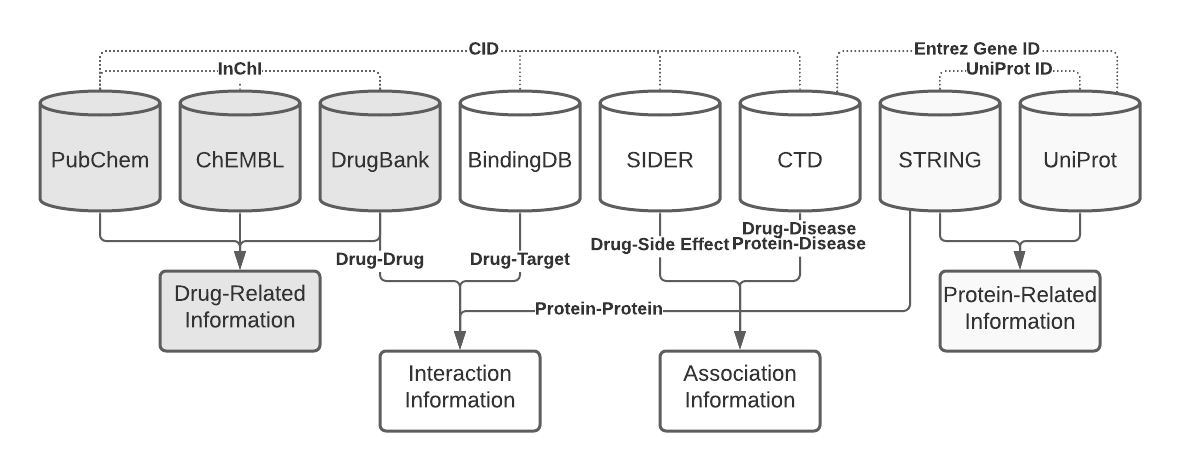
\includegraphics[width=\linewidth]{chapters/materials_and_methods/figures/databases.png}
    \caption{Compiled Databases.}
    \label{fig:databases}
\end{figure}

\section{Dataset Preparation}
% TO DO: Which information is used, jaccard vs also, lm

\section{Graph Creation}
% TO DO: Insert node edge numbers, types
% pos and neg edge sampling

\section{Learning Distributional Vector Representations}
Machine learning on graph structured data is a ubiquitous task and one of the challenges of this task is to find a way to represent the structure itself and the information it holds so that it can be easily interpreted by mostly used machine learning models. In this thesis, we employ MetaPath2Vec \cite{dong2017metapath2vec} model and learn the graph-based distributional representation vectors that reflect the semantic connections in the graph for nodes and edges and finally represent data that cannot be expressed in Euclidean space as a graph.

MetaPath2Vec uses \textit{priori} paths as its basic operating principle. It evaluates different types of edge relations while finding meta paths, that is, paths going from one node to another node, provided that they do not repeat it again, and makes semantic inferences using these edges and uses them in vector representations.



% Explain metapath2vec in short. 
% cosine similarity ile val evaluation
% hepsinin sonuclari



\section{WiderDeepDTA}
% degisen kisimlari acikla
